% ==============================================================================
% Chapter 9: V–A Structure from 5D Chiral Localization
% Status: [Dc] — Derived from 5D Dirac + EDC postulates
% ==============================================================================

% Chapter intro (no section number)
\label{sec:ch9_va_structure}

\begin{tcolorbox}[edcGuardrail, title=\textbf{Epistemic Status}]
This section derives the effective 4D V–A (left-chiral) current structure
from the EDC 5D$\to$4D reduction. The derivation uses:
\begin{itemize}[nosep]
    \item Standard 5D Dirac equation with position-dependent mass \tagBL{}
    \item Domain-wall zero mode localization~\cite{JackiwRebbi1976,Kaplan1992} \tagBL{}
    \item EDC postulate: Plenum inflow determines mass profile sign \tagP{}
    \item Geometric domain: half-line $\xi \in [0, \infty)$ \tagP{}
    \item Interaction locality: gauge fields live at the boundary \tagP{}
\end{itemize}
The result---that only left-handed modes couple at the interface---is
\textbf{derived-conditional} \tagDc{}: it follows \emph{mathematically} from
the above assumptions, but those assumptions include postulates \tagP{} that
are not themselves derived. The V--A structure is robust against details of
the mass profile $m(\xi)$ as long as $m(\xi) > 0$ for $\xi > 0$.
\end{tcolorbox}

% ==============================================================================
% FRAMEWORK 2.0 LANGUAGE COMPLIANCE
% ==============================================================================
\begin{tcolorbox}[colback=blue!3!white, colframe=blue!50!black,
    title=\textbf{Framework 2.0 Language Compliance}]
\small
\textbf{EDC Projection Principle:} Every physical process has a \textbf{5D bulk+brane cause}
whose observable residue is a \textbf{3D shadow} on the observer boundary.

\textbf{In this chapter:}
\begin{itemize}[nosep]
    \item \textbf{5D cause:} Plenum inflow creates directional mass gradient $m(\xi) > 0$ for $\xi > 0$.
    \item \textbf{Brane process:} Chiral mode localization via domain-wall mechanism.
    \item \textbf{3D shadow:} V--A current structure observed in weak decays.
\end{itemize}

\textbf{Standard Model terms} (e.g., ``$V{-}A$ current,'' ``weak interaction'') appear as
\textbf{3D observational shorthand}, not as primary causes. The SM accurately describes
\emph{what} 4D observers measure; EDC explains \emph{why} it takes that form.
\end{tcolorbox}

% ==============================================================================
\section{The Physical Picture: What Happens in 5D?}
\label{sec:ch9_physical_picture}

% --- PHYSICAL PROCESS SUMMARY (Feynman-style) ---
\begin{tcolorbox}[colback=green!5!white, colframe=green!50!black,
    title=\textbf{The V--A Mechanism in One Paragraph}]
The 5D universe has a depth coordinate $\xi$; observers live on a brane at $\xi = 0$.
A sign-changing mass term---induced by Plenum inflow---acts as a \textbf{chirality
filter}: the left-handed zero-mode wavefunction $f_L(\xi)$ clings to the boundary
(exponentially localized at $\xi = 0$), while the right-handed wavefunction $f_R(\xi)$
is displaced into the bulk (either non-normalizable on the half-line, or
exponentially suppressed at the boundary on a compact interval). Weak interactions
``happen where the gauge field lives''---in the minimal embedding, at the brane.
Therefore, coupling strength is controlled by \textbf{boundary overlap}: $f_L$ has
$\mathcal{O}(1)$ overlap $\Rightarrow$ full coupling; $f_R$ has suppressed overlap
$\Rightarrow$ negligible coupling. The result: effective V--A emerges from geometry,
not from imposing chirality by hand \tagDc{}.
\end{tcolorbox}

\medskip
Before writing any equations, let us watch the ``movie'' of what happens in the
fifth dimension. This subsection gives the physical story; the mathematical
derivation follows in subsequent sections.

% --- THE MOVIE ---

\subsection{The Setup: A Universe with Depth}

Imagine you are a 4D observer living on a thin membrane---the ``brane''---embedded
in a larger 5D space. You cannot travel into the fifth dimension $\xi$, but particles
can have profiles that extend into it.

\textbf{What is $\xi$?} The coordinate $\xi$ measures distance perpendicular to the
brane. At $\xi = 0$ sits the observer boundary---the surface where we make measurements.
As $\xi$ increases, we move ``into the bulk,'' away from observer space.

\textbf{What is the brane?} The brane is a 4D hypersurface where ordinary matter
is localized. Think of it as the floor of a swimming pool: particles are waves
on the surface, but the pool has depth ($\xi > 0$).

\textbf{What does an observer see?} A 4D observer sees only the ``shadow'' of
5D fields projected onto the boundary. The strength of a particle's interaction
depends on how much of its wavefunction sits at the boundary.

% --- CHIRALITY FILTER ---

\subsection{The Chirality Filter: Why Only Left-Handed?}

Here is the key physical insight, stated in one sentence:

\begin{center}
\fbox{\parbox{0.85\textwidth}{\centering
\textbf{The chirality filter:} Left-handed modes are pulled toward the boundary
by the 5D mass gradient; right-handed modes are pushed away into the bulk.
}}
\end{center}

Why does this happen? The mechanism is elegantly simple:

\textbf{Step 1: Energy flows inward.} In EDC, the Plenum (the 5D energy fluid)
flows toward the observer boundary. This is the fundamental asymmetry that
breaks left-right symmetry.

\textbf{Step 2: The inflow creates a mass gradient.} The flowing Plenum exerts
stress on fermion fields. Near the boundary, fermions feel less stress; deeper
in the bulk, they feel more. This creates a position-dependent mass $m(\xi)$ that
grows with depth.

\textbf{Step 3: The mass gradient acts like a potential.} A left-handed fermion
in this background experiences an effective force \emph{toward} the boundary
(like a ball rolling downhill). A right-handed fermion experiences a force
\emph{away} from the boundary (like trying to push a ball uphill---it rolls away).

\textbf{Step 4: Localization follows.} Left-handed modes pile up at $\xi = 0$;
right-handed modes spread into the bulk and become dilute.

% --- OVERLAP AND COUPLING ---

\subsection{Overlap Determines Coupling}

Now we can understand why left-handed particles interact and right-handed
particles do not.

\textbf{The principle:} Interaction strength equals wavefunction overlap at the
boundary.

Imagine two flashlights shining on a single screen: the overlap of their beams
determines how much they interact. Similarly, if a gauge boson (like the $W$)
lives at the boundary, it can only ``see'' the part of a fermion wavefunction
that also lives there.

\textbf{Left-handed fermions:} Their wavefunction $f_L(\xi)$ is peaked at $\xi = 0$.
Most of the probability density sits right at the boundary. The overlap with
a boundary-localized gauge field is order one: full coupling.

\textbf{Right-handed fermions:} Their wavefunction $f_R(\xi)$ is peaked deep in
the bulk. Only an exponentially small tail reaches the boundary. The overlap
is exponentially suppressed: negligible coupling.

This is the geometric origin of parity violation in weak interactions.

% --- WHAT WE DERIVE VS NOT ---

\subsection{What We Derive and What We Do Not}

\begin{tcolorbox}[colback=blue!5, colframe=blue!50!black,
    title=\textbf{Scope of This Chapter}]

\textbf{What this chapter DERIVES} \tagDc{}:
\begin{itemize}[nosep]
    \item Left-handed modes are boundary-localized
    \item Right-handed modes are bulk-displaced
    \item Effective weak coupling is purely V$-$A
    \item Chirality selection follows from inflow direction, not gauge assignments
\end{itemize}

\textbf{What this chapter does NOT derive} (open):
\begin{itemize}[nosep]
    \item The origin of SU(2)$_L$ gauge symmetry---why this particular group?
    \item The W$^\pm$ and Z$^0$ boson masses---Higgs mechanism not addressed
    \item The numerical value of $G_F$---see Chapter 11
    \item CKM/PMNS mixing matrices---generational structure not derived
    \item Neutrino masses and Dirac vs.\ Majorana nature
\end{itemize}

\textbf{Epistemic tags:}
\begin{itemize}[nosep]
    \item Plenum inflow direction: \tagP{} (EDC postulate)
    \item Mass-from-stress coupling: \tagP{} (physical hypothesis)
    \item Domain-wall localization math: \tagBL{} (established physics)
    \item V$-$A emergence from localization: \tagDc{} (derived here)
\end{itemize}
\end{tcolorbox}

% ==============================================================================
\section{Purpose and Scope}
\label{sec:ch9_purpose}

With the physical picture in mind, we now state the mathematical problem.

\subsection{The 3D Observation (What Observers See)}

From the 3D observer's vantage point, the weak interaction couples exclusively
to left-handed fermions. The effective 4D description is the $V{-}A$ current:
\begin{equation}
    \mathcal{L}_{\text{weak}} \propto \bar\psi \gamma^\mu (1 - \gamma^5) \psi \, W_\mu
    \label{eq:ch9_va_current}
\end{equation}
This is the \emph{observed 3D shadow} \tagBL{}. The EDC question is: what 5D
cause produces this shadow?

\subsection{The 3D Observational Description (SM)}

From the 3D observer's perspective, the Standard Model describes what is
measured: left-right asymmetry is encoded via gauge quantum number assignments
($\psi_L$ doublets, $\psi_R$ singlets under SU(2)$_L$). This description is
\emph{accurate}---it correctly parametrizes the 3D shadow \tagBL{}. However,
it does not explain \emph{why} chirality selection occurs; it encodes the
observation as input.

\subsection{The EDC Approach: 5D Cause → 3D Shadow}

In EDC, chirality selection is a \emph{consequence} of 5D geometry: the 3D
observer sees V--A because that is the shadow cast by Plenum-induced mode
localization in the extra dimension. The asymmetry arises from physics---the
directional inflow---not from ad hoc quantum number assignments.

\paragraph{Minimal assumptions.}
We use only:
\begin{enumerate}[nosep]
    \item The 5D Dirac equation with $\xi$-dependent mass $m(\xi)$ \tagBL{}
    \item The EDC postulate that Plenum flows toward the observer boundary \tagP{}
    \item The physical coupling of fermion mass to Plenum stress \tagP{}
\end{enumerate}

\paragraph{Geometric domain choice \tagP{}.}
\textbf{Throughout this chapter we work on the half-line $\xi \in [0, \infty)$} with
the observer boundary at $\xi = 0$ and the bulk extending to $\xi \to \infty$.
Alternative domains (finite interval $[0, \ell]$, orbifold $S^1/\mathbb{Z}_2$)
would require modified boundary conditions and could change the spectrum of
normalizable modes. The half-line choice is the simplest setting that exhibits
the chirality filter mechanism; finite-interval or orbifold variants are
deferred to Chapter~\ref{ch:bvp_master_key} (BVP Work Package).

% --- LOCAL VS GLOBAL GEOMETRY MAP ---
\begin{tcolorbox}[colback=blue!5!white, colframe=blue!50!black,
    title=\textbf{Local vs Global Geometry Map}]
\textbf{This chapter is a LOCAL near-brane analysis} \tagP{}. The half-line
domain $\xi \in [0, \infty)$ captures the physics close to the observer boundary
where the chirality filter operates. This is sufficient to establish the V--A
mechanism.

\textbf{Chapters that compute spectra and masses} (Ch.~11, OPR-20) use
\textbf{GLOBAL compact geometries}: finite intervals $[0, \ell]$ or orbifolds
$S^1/\mathbb{Z}_2$. That is a different modeling layer \tagDc{}.

\textbf{Relationship:}
\begin{itemize}[nosep]
    \item \textbf{Local (this chapter):} Chiral localization + overlap suppression
          $\Rightarrow$ V--A selection. \tagDc{}
    \item \textbf{Global (Ch.~11/OPR-20):} KK tower, eigenvalues $x_1$, mediator
          mass spectrum. \tagDc{}
    \item \textbf{Bridge:} The same fermion profiles $f_{L/R}(z)$ enter both
          analyses; the global BVP supplies the compactification scale $\ell$
          and eigenvalue $x_1$. \tagDc{}
\end{itemize}

\textbf{Bottom line:} V--A selection is robust at the local level; exact mediator
masses require the global KK boundary value problem \tagDc{}.
\end{tcolorbox}

\paragraph{Scope and limitations.}
\begin{itemize}[nosep]
    \item This chapter addresses chirality selection, not SU(2)$_L$ gauge unification.
    \item CKM/PMNS mixing is not derived here; it remains (open).
    \item The numerical value of $G_F$ is not computed; see Ch.~11 for the pathway.
\end{itemize}

% ==============================================================================
\section{5D Dirac Field and Chiral Decomposition}
\label{sec:ch9_dirac}

We now write the equations. Remember: these equations \emph{formalize} the
physical picture from Section~\ref{sec:ch9_physical_picture}, not replace it.

\subsection{The 5D Dirac Equation}

\textbf{The setup.} Consider a fermion field $\Psi(x^\mu, \xi)$ in the 5D EDC geometry.
The coordinates are $x^M = (x^\mu, \xi)$ where $\mu = 0,1,2,3$ and $\xi$ is
the fifth dimension (perpendicular to the brane).

\textbf{The equation.} The 5D Dirac equation with position-dependent mass is \tagBL{}:
\begin{equation}
    \left( i\gamma^\mu \partial_\mu + i\gamma^5 \partial_\xi - m(\xi) \right) \Psi = 0
    \label{eq:ch9_5d_dirac}
\end{equation}
This is the standard Dirac equation, except that the mass is not a constant---it
depends on where you are in the fifth dimension.

\textbf{What each term does:}
\begin{itemize}[nosep]
    \item $\gamma^\mu$ are the standard 4D Dirac matrices, $\{\gamma^\mu, \gamma^\nu\} = 2\eta^{\mu\nu}$
    \item $\gamma^5 = i\gamma^0\gamma^1\gamma^2\gamma^3$ is the chirality operator
    \item $m(\xi)$ is the position-dependent fermion mass (to be determined by EDC physics)
\end{itemize}

The key is the term $i\gamma^5 \partial_\xi$: it couples left-handed and right-handed
components differently to the $\xi$-direction. This is where chirality enters.

\subsection{Chiral Projection Operators}

\textbf{The definition.} We split any spinor into left-handed and right-handed parts.
Define the 4D chiral projectors \tagBL{}:
\begin{equation}
    P_L = \frac{1}{2}(1 - \gamma^5), \qquad P_R = \frac{1}{2}(1 + \gamma^5)
    \label{eq:ch9_projectors}
\end{equation}
These satisfy $P_L + P_R = 1$, $P_L P_R = 0$, and $\gamma^5 P_{L/R} = \mp P_{L/R}$.

\textbf{The decomposition.} Any spinor splits cleanly into two pieces:
\begin{equation}
    \Psi(x,\xi) = \Psi_L(x,\xi) + \Psi_R(x,\xi), \qquad \Psi_{L/R} = P_{L/R} \Psi
    \label{eq:ch9_decomposition}
\end{equation}
Think of $\Psi_L$ and $\Psi_R$ as two species of particle that can transform into
each other through the mass term.

\subsection{Mode Expansion}

\textbf{Zero-mode limit.} The equations below correspond to the \textbf{chiral
zero-mode limit} where the 4D mass eigenvalue $m_4 = 0$. For massive 4D modes
($m_4 \neq 0$), the left- and right-handed profiles couple through the 4D mass
term, leading to a second-order Schrödinger-like eigenvalue problem (see the
BVP work package, Chapter~\ref{ch:bvp_master_key}). The zero-mode analysis captures the leading
chirality-selection mechanism; massive-mode corrections are higher-order.

\medskip
\textbf{Separating variables.} We want to find how the left- and right-handed
pieces are distributed in $\xi$. For a massless 4D mode with momentum $p_\mu$, write:
\begin{equation}
    \Psi(x,\xi) = \psi_L(x) f_L(\xi) + \psi_R(x) f_R(\xi)
    \label{eq:ch9_mode_expansion}
\end{equation}
Here $\psi_{L/R}(x)$ are 4D spinor fields and $f_{L/R}(\xi)$ are $\xi$-profiles.
The profiles tell us: how much of each chirality lives at each depth?

\textbf{The profile equations.} Substituting into Eq.~\eqref{eq:ch9_5d_dirac} and
separating chiralities gives the coupled first-order equations \tagBL{}:
\begin{align}
    \partial_\xi f_L &= -m(\xi) f_L \label{eq:ch9_fL_eq} \\
    \partial_\xi f_R &= +m(\xi) f_R \label{eq:ch9_fR_eq}
\end{align}
Notice the crucial sign difference: $f_L$ gets a minus sign, $f_R$ gets a plus sign.

\textbf{What this means physically:} If $m(\xi) > 0$, then $f_L$ decreases with $\xi$
(the left-handed mode is pushed toward smaller $\xi$), while $f_R$ increases with $\xi$
(the right-handed mode is pushed toward larger $\xi$).

\textbf{The formal solutions.} These first-order equations integrate immediately:
\begin{align}
    f_L(\xi) &= f_L(0) \exp\left(-\int_0^\xi m(\xi') \, d\xi'\right) \label{eq:ch9_fL_sol} \\
    f_R(\xi) &= f_R(0) \exp\left(+\int_0^\xi m(\xi') \, d\xi'\right) \label{eq:ch9_fR_sol}
\end{align}
The left-handed profile is an exponentially \emph{decaying} function of depth.
The right-handed profile is an exponentially \emph{growing} function of depth.

% ==============================================================================
\section{Interface Mass Profile and Localization}
\label{sec:ch9_localization}

We have the equations for the profiles. Now we need the mass function $m(\xi)$.
This is where EDC physics enters.

\subsection{The Domain Wall Mechanism (Baseline)}

First, let us recall what is already known from standard physics \tagBL{}.

\textbf{The Jackiw--Rebbi--Kaplan mechanism.} The localization of chiral fermions
at domain walls is a well-known result~\cite{JackiwRebbi1976,Kaplan1992}:
\begin{itemize}[nosep]
    \item If $m(\xi)$ increases from negative to positive values (e.g., $m(\xi) = m_0 \tanh(z/L)$),
          then the \textbf{left-handed} zero mode is localized at $\xi = 0$.
    \item If $m(\xi)$ decreases from positive to negative, the \textbf{right-handed}
          mode is localized.
\end{itemize}

\textbf{The physics:} The sign of the mass profile determines chirality selection.
Whichever chirality is ``uphill'' in the mass landscape gets pushed to the minimum.

\subsection{EDC Postulate: Plenum Inflow Determines Mass Sign}

Now we add the EDC ingredient. In EDC, the Plenum (5D energy fluid) flows toward
the observer boundary:
\begin{equation}
    J^z_{\text{Plenum}} > 0 \qquad \text{(inflow toward $\xi = 0$)}
    \label{eq:ch9_inflow}
\end{equation}
This is the fundamental EDC mechanism (see Framework v2.0, Remark~4.5) \tagP{}.

\textbf{Why does this matter?} The inflow creates a directional asymmetry in
the 5D geometry. The bulk and the boundary are not equivalent---energy flows
from one to the other.

\begin{tcolorbox}[colback=orange!5, colframe=orange!50!black,
    title=\textbf{Physical Hypothesis [P]}]
\textbf{The idea:} The fermion mass $m(\xi)$ is induced by coupling to the Plenum
stress tensor. Where the energy flow is stronger, the effective mass is larger.
\begin{equation}
    m(\xi) \sim \kappa \left( T^{zz}(z) - T^{zz}(0) \right)
    \label{eq:ch9_mass_from_stress}
\end{equation}
where $\kappa > 0$ is a coupling constant.

\textbf{Physical interpretation:} A fermion feels ``heavier'' where the Plenum
flow exerts more pressure. The boundary is a low-pressure region; the bulk
is a high-pressure region.
\end{tcolorbox}

\textbf{The consequence.} Since Plenum flows inward, the stress $T^{zz}$ is
larger in the bulk than at the boundary:
\begin{equation}
    T^{zz}(z) > T^{zz}(0) \quad \text{for } \xi > 0
    \qquad\Longrightarrow\qquad
    m(\xi) > 0 \quad \text{for } \xi > 0
    \label{eq:ch9_mass_positive}
\end{equation}

\textbf{The profile.} The resulting mass profile is a ``half-domain wall'':
\begin{equation}
    m(\xi) = m_0 \left(1 - e^{-z/\lambda}\right) \approx m_0 \frac{z}{\lambda}
    \quad \text{for small } z
    \label{eq:ch9_mass_profile}
\end{equation}
where $\lambda$ is the characteristic length scale (related to thick-brane
thickness $\Delta$).

\textbf{The picture:} Mass is zero at the boundary and grows into the bulk.
This is not a symmetric domain wall---it is a ``ramp'' starting at zero.

\subsection{Chiral Mode Profiles}

Now we can solve for the profiles explicitly.

With $m(\xi) > 0$ for $\xi > 0$, the profile equations~\eqref{eq:ch9_fL_sol}--\eqref{eq:ch9_fR_sol} give:

\paragraph{Left-handed mode.}
\begin{equation}
    f_L(\xi) = N_L \exp\left(-\int_0^\xi m(\xi') \, d\xi'\right)
    \label{eq:ch9_fL_profile}
\end{equation}

\textbf{What happens:} Since $m(\xi') > 0$ for all $\xi' > 0$, the integral
$\int_0^\xi m(\xi') d\xi'$ is positive and grows with $\xi$. Therefore $f_L(\xi)$
\textbf{decreases} as $\xi$ increases.

\textbf{The result:} The left-handed mode is \textbf{localized at the boundary}
$\xi = 0$ \tagDc{}. It piles up where we make measurements.

\paragraph{Right-handed mode.}
\begin{equation}
    f_R(\xi) = N_R \exp\left(+\int_0^\xi m(\xi') \, d\xi'\right)
    \label{eq:ch9_fR_profile}
\end{equation}

\textbf{What happens:} The positive sign in the exponent causes $f_R(\xi)$ to
\textbf{grow} as $\xi$ increases.

\textbf{The result (half-line):} On the half-line domain, this mode is
\textbf{not normalizable}; it is expelled into the bulk \tagDc{}. It runs away
from the boundary.\footnote{Normalizability conditions depend on the chosen
domain. On a finite interval or orbifold, $f_R$ can be normalizable but its
overlap at the boundary remains exponentially suppressed---the V--A mechanism
persists. \tagDc{}}

\subsection{Normalizability Conditions (Domain-Dependent)}

\textbf{Why normalizability matters.} A physical mode must have finite probability:
$\int |f(\xi)|^2 \, d\xi < \infty$. Whether a profile is normalizable depends on
both the mass function $m(\xi)$ and the domain.

\paragraph{Half-line domain ($\xi \in [0, \infty)$).}
On the half-line (our working assumption), normalizability requires:
\begin{itemize}[nosep]
    \item $f_L$: Normalizable if $\int_0^\infty m(z')\,d\xi' \to +\infty$ as $\xi \to \infty$
          (the integral diverges, so $f_L \to 0$ fast enough).
    \item $f_R$: \textbf{Not normalizable} because the exponential grows without bound.
\end{itemize}
With $m(\xi) > 0$ for all $\xi > 0$, the left-handed mode is the \emph{only} normalizable
zero mode.

\paragraph{Finite interval ($\xi \in [0, \ell]$).}
On a finite interval, both profiles are formally normalizable (integrals are finite).
However, the boundary conditions at $\xi = \ell$ determine which modes survive:
\begin{itemize}[nosep]
    \item \textbf{Dirichlet at both ends:} Discrete spectrum; chirality selection
          depends on mode number parity.
    \item \textbf{Orbifold ($S^1/\mathbb{Z}_2$):} Reflection symmetry can project
          out one chirality entirely.
\end{itemize}
The finite-interval case is addressed in the BVP work package (Chapter~\ref{ch:bvp_master_key}).

\begin{center}
\fbox{\parbox{0.9\textwidth}{
\textbf{Key result:} With the EDC mass profile (positive, rising into bulk)
on the half-line domain, only left-handed modes are localized at the observer
boundary. Right-handed modes delocalize into the bulk and do not participate in
brane-localized interactions.
}}
\end{center}

% ==============================================================================
\section{Toy Model: Overlap Suppression}
\label{sec:ch9_toy_model}

The previous sections gave exact solutions. Now let us build physical intuition
with a simple toy model. The goal is to see \emph{how much} the right-handed
coupling is suppressed, without using Standard Model numbers.

\begin{tcolorbox}[colback=gray!5, colframe=gray!50!black,
    title=\textbf{Toy Model Disclaimer}]
This subsection contains \textbf{new} equations that illustrate the overlap
mechanism. These are \tagP{} toy-model assumptions, not derived from first
principles. The purpose is pedagogical: to show how exponential suppression
emerges from simple profiles.
\end{tcolorbox}

\subsection{Simple Profile Ansatz [P]}

For the toy model, assume Gaussian profiles for the fermion modes:

\textbf{Left-handed profile} (localized at boundary):
\begin{equation}
    f_L^{\text{(toy)}}(z) = \frac{1}{(\pi w_L^2)^{1/4}} \exp\left(-\frac{z^2}{2w_L^2}\right)
    \label{eq:ch9_toy_fL}
\end{equation}
This is peaked at $\xi = 0$ with width $w_L$.

\textbf{Right-handed profile} (displaced into bulk):
\begin{equation}
    f_R^{\text{(toy)}}(z) = \frac{1}{(\pi w_R^2)^{1/4}} \exp\left(-\frac{(z - z_0)^2}{2w_R^2}\right)
    \label{eq:ch9_toy_fR}
\end{equation}
This is peaked at $\xi = z_0 > 0$ with width $w_R$.

\textbf{Physical meaning of parameters:}
\begin{itemize}[nosep]
    \item $w_L$: width of left-handed wavefunction (how ``spread out'' it is)
    \item $w_R$: width of right-handed wavefunction
    \item $z_0$: displacement of right-handed mode into bulk
\end{itemize}

\subsection{Overlap Integral [Dc conditional on toy ansatz]}

The effective coupling of a chirality to a boundary-localized gauge field is
proportional to the wavefunction value at $\xi = 0$:

\textbf{Left-handed coupling:}
\begin{equation}
    g_L^{\text{(toy)}} \propto |f_L^{\text{(toy)}}(0)|^2 = \frac{1}{\sqrt{\pi} w_L}
    \label{eq:ch9_toy_gL}
\end{equation}
This is $\mathcal{O}(1)$ for $w_L \sim 1$ in natural units.

\textbf{Right-handed coupling:}
\begin{equation}
    g_R^{\text{(toy)}} \propto |f_R^{\text{(toy)}}(0)|^2
    = \frac{1}{\sqrt{\pi} w_R} \exp\left(-\frac{z_0^2}{w_R^2}\right)
    \label{eq:ch9_toy_gR}
\end{equation}

\textbf{The suppression factor:}
\begin{equation}
    \frac{g_R^{\text{(toy)}}}{g_L^{\text{(toy)}}} \sim \exp\left(-\frac{z_0^2}{w_R^2}\right)
    \label{eq:ch9_toy_suppression}
\end{equation}

\subsection{Physical Interpretation}

\textbf{What does this tell us?}

The ratio of right-handed to left-handed coupling is exponentially suppressed
by the factor $(z_0/w_R)^2$.

\begin{itemize}[nosep]
    \item If $z_0 \gg w_R$ (displacement much larger than width), the suppression
          is enormous: $g_R/g_L \sim e^{-\text{large}}$.
    \item If $z_0 \sim w_R$, there is moderate suppression: $g_R/g_L \sim e^{-1}$.
    \item If $z_0 \ll w_R$, there is little suppression: the modes overlap.
\end{itemize}

\textbf{For V$-$A to work}, we need $z_0 \gg w_R$: the right-handed mode must
be displaced far enough that its tail at the boundary is negligible.

\textbf{This is exactly what the EDC mass profile achieves:} the growing mass
$m(\xi)$ pushes the right-handed mode deep into the bulk, making $z_0$ large.

% ==============================================================================
\subsection{Quantitative Suppression Target (Inequality Chain, No Calibration)}
\label{subsec:va_inequality_chain}

The previous subsection gave qualitative suppression. Here we state the
\emph{quantitative closure target}: what suppression level is required for
consistency with experiment, and what parameter regime must hold.

\begin{tcolorbox}[colback=yellow!5!white, colframe=yellow!60!black,
    title=\textbf{Epistemic Status: Closure Target, Not Calibration}]
\label{box:va_inequality_status}

\textbf{What this section provides:}
\begin{itemize}[nosep]
    \item The empirical bound on RH current admixture (3D baseline)
    \item The inequality chain that constrains the dimensionless barrier parameter
    \item The closure target: what must be derived, not assumed
\end{itemize}

\textbf{What this section does NOT do:}
\begin{itemize}[nosep]
    \item Derive the barrier parameter from membrane physics (remains OPEN)
    \item Tune parameters to match the bound (no calibration)
    \item Claim closure of the V--A mechanism quantitatively
\end{itemize}
\end{tcolorbox}

\subsubsection{The Chirality Ratio (Definition)}

\begin{definition}[Chirality Asymmetry Ratio]
\label{def:va:RLR}
\tagDef{}
The \textbf{chirality asymmetry ratio} $R_{\text{LR}}$ quantifies the relative
coupling of right-handed modes to the brane:
\begin{equation}
    R_{\text{LR}} \equiv \frac{|f_R(0)|^2}{|f_L(0)|^2}
    = \frac{g_{\text{eff}}^{(R)}}{g_{\text{eff}}^{(L)}}
    \label{eq:va:RLR_def}
\end{equation}
where $f_{L/R}(0)$ are the chiral mode profiles evaluated at the brane boundary.
\end{definition}

For the exact solutions~\eqref{eq:ch9_fL_sol}--\eqref{eq:ch9_fR_sol}, if we set
boundary normalizations $f_L(0) = f_R(0)$, then:
\begin{equation}
    R_{\text{LR}} = \exp\left(-2\int_0^{\xi_*} m(\xi')\,d\xi'\right)
    \label{eq:va:RLR_exact}
\end{equation}
where $\xi_*$ is a characteristic depth (e.g., where the RH mode peaks, or the
domain cutoff).

\subsubsection{The 3D Empirical Baseline}

Experiments constrain right-handed currents in weak decays. The Standard Model
is built on purely left-handed charged currents; any RH admixture is tightly
bounded~\cite{PDG2024}:
\begin{equation}
    R_{\text{LR}}^{\text{(exp)}} < 10^{-3}
    \qquad \text{(3D empirical baseline \tagBL{})}
    \label{eq:va:empirical_bound}
\end{equation}
This bound comes from precision measurements of parity violation in nuclear
and particle physics. The weak interaction is \emph{almost purely} V$-$A;
any V$+$A component is suppressed by at least three orders of magnitude.

\subsubsection{The Inequality Chain}

From the exponential form~\eqref{eq:va:RLR_exact}, define a dimensionless
\textbf{barrier parameter}:
\begin{equation}
    \mu \equiv \int_0^{z_*} \frac{m(z')}{\Lambda}\,d\xi'
    \label{eq:va:mu_def}
\end{equation}
where $\Lambda$ is a characteristic mass scale (e.g., $m_0$ or $1/\lambda$ from
the profile). The localization mechanism implies exponential suppression:
\begin{equation}
    R_{\text{LR}} \sim e^{-C\mu}
    \label{eq:va:RLR_mu}
\end{equation}
where $C > 0$ is a \emph{model-dependent} $\mathcal{O}(1)$ coefficient determined
by the detailed shape of the profile/potential and admissible boundary conditions.
The coefficient $C$ is \tagOPEN{} until $V(\xi)$ and BCs are derived from the 5D action.
\textbf{Update:} The potential structure $V_L, V_R$ and Robin BCs have been derived in
\S\ref{subsec:opr21_closure} (Ch.~14); $C$ remains model-dependent via the profile shape.

\paragraph{The suppression inequality (parameter-free form).}
Combining Eqs.~\eqref{eq:va:empirical_bound} and \eqref{eq:va:RLR_mu} yields
the \emph{parameter-free} inequality target:
\begin{equation}
    \boxed{
    \mu > \frac{1}{C}\ln(10^3)
    \qquad
    \text{with } C = \mathcal{O}(1) \Rightarrow \mu = \mathcal{O}(5\text{--}10)
    }
    \label{eq:va:mu_bound}
\end{equation}
This is the \textbf{closure target}: the barrier parameter must lie in a robust
$\mathcal{O}(5\text{--}10)$ regime for generic $C = \mathcal{O}(1)$.%
\footnote{Illustration only (Toy): if one takes $C \simeq 2$, then
Eq.~\eqref{eq:va:mu_bound} gives $\mu \gtrsim 3.45$. This is not a fit and does
not close the claim; it only shows the scaling.}
We do \emph{not} assume $C$; the only claim is the inequality target.
Determining $C$ is delegated to the BVP closure pack (OPR-21, Ch.~14).

\paragraph{Interpretation.}
\begin{itemize}[nosep]
    \item $\mu$ measures the ``cumulative mass barrier'' the RH mode must cross
          to reach the brane.
    \item $\mu = \mathcal{O}(5\text{--}10)$ is a modest requirement---roughly
          5--10 $e$-foldings in the wavefunction before it becomes negligible
          (depending on $C$).
    \item For a linear mass profile $m(\xi) = m_0 z/\lambda$, this requires
          $m_0 z_*/\lambda = \mathcal{O}(5\text{--}10)$, i.e., the characteristic
          depth must be several times the localization scale.
\end{itemize}

\subsubsection{What Must Be Derived (OPEN)}

\begin{tcolorbox}[colback=red!5!white, colframe=red!50!black,
    title=\textbf{Closure Condition: Derive $\mu$ from Membrane Parameters}]
\label{box:va_mu_closure}

\textbf{Status:} \tagOPEN{}

The barrier parameter $\mu$ depends on:
\begin{enumerate}[nosep]
    \item The mass profile $m(\xi)$, which must be derived from Plenum-fermion
          coupling (Sec.~\ref{sec:ch9_localization})
    \item The integration cutoff $z_*$, which depends on domain geometry
          (half-line vs finite interval)
    \item The scale $\Lambda$, which must connect to membrane parameters
          $(\sigma, r_e, R_\xi)$
\end{enumerate}

\textbf{Closure requires:}
\begin{itemize}[nosep]
    \item Express $\mu$ and $C$ in terms of $(\sigma, r_e)$ from Part~I
    \item Show $\mu > \ln(10^3)/C$ follows from membrane physics, not from tuning
    \item Verify robustness under domain and BC variations
\end{itemize}

\textbf{Without this derivation:} V--A is qualitatively established but
quantitative suppression remains a postulated regime \tagP{}.
\end{tcolorbox}

\subsubsection{Connection to BVP Closure Pack}

The chirality asymmetry ratio $R_{\text{LR}}$ is defined in the BVP closure
pack (Ch.~14, Definition~\ref{def:bvp:chirality}). The overlap integrals
$I_4$ and related quantities can be computed once the BVP is solved with
a derived $V(\xi)$.

\paragraph{Cross-references.}
\begin{itemize}[nosep]
    \item BVP closure pack: Ch.~14, Sec.~\ref{subsec:bvp_outputs}
    \item Chirality suppression criterion: Ch.~14, Sec.~\ref{subsubsec:bvp_chirality}
    \item $V(\xi)$ candidates catalogue: Ch.~14, Sec.~\ref{subsec:bvp_vz_catalogue}
\end{itemize}

\begin{tcolorbox}[colback=green!5!white, colframe=green!60!black,
    title=\textbf{Reader Takeaway: Not a Fit, but a Closure Target}]
\label{box:va_takeaway}

This subsection does \emph{not} fit parameters to achieve $R_{\text{LR}} < 10^{-3}$.
Instead, it states:
\begin{enumerate}[nosep]
    \item The empirical baseline: $R_{\text{LR}} < 10^{-3}$ from experiment \tagBL{}
    \item The mathematical consequence: $\mu \gtrsim 3.5$ (barrier parameter)
    \item The closure target: derive $\mu$ from membrane physics \tagOPEN{}
\end{enumerate}

\textbf{This is the required regime for the mechanism to match the empirical
baseline.} If the derived membrane parameters yield $\mu < 3.5$, the model
would be in tension with experiment. If $\mu \gg 3.5$, the suppression is
stronger than required (consistent, but not a prediction).

The goal is to show that membrane physics \emph{naturally} produces $\mu \gtrsim 3.5$,
not to choose $\mu$ to make V--A work.
\end{tcolorbox}

% --- FIGURE PLACEHOLDER ---

\subsection{Schematic Visualization}

\begin{figure}[htbp]
\centering
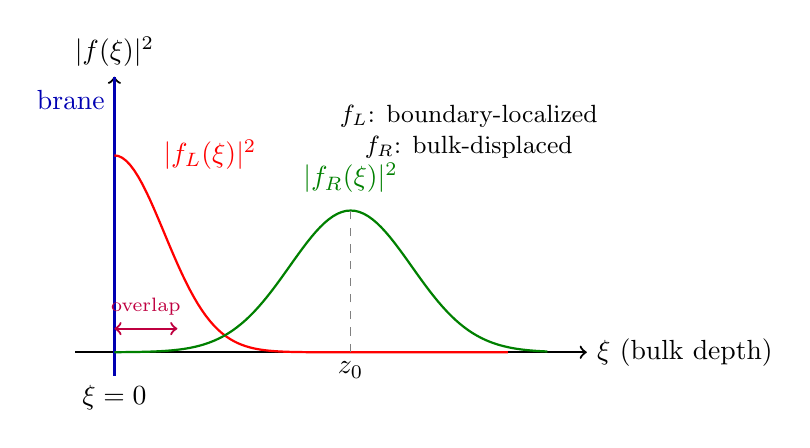
\begin{tikzpicture}[scale=1.0]
    % Axes
    \draw[->, thick] (-0.5,0) -- (6,0) node[right] {$\xi$ (bulk depth)};
    \draw[->, thick] (0,-0.3) -- (0,3.5) node[above] {$|f(\xi)|^2$};

    % Brane at \xi = 0
    \draw[very thick, blue!70!black] (0,-0.3) -- (0,3.5);
    \node[blue!70!black, left] at (0,3.2) {brane};
    \node[below] at (0,-0.3) {$\xi = 0$};

    % Left-handed profile (peaked at \xi = 0)
    \draw[thick, red, domain=0:5, samples=100]
        plot (\x, {2.5*exp(-\x*\x/0.8)});
    \node[red, above right] at (0.5,2.2) {$|f_L(\xi)|^2$};

    % Right-handed profile (peaked at z=z_0)
    \draw[thick, green!50!black, domain=0:5.5, samples=100]
        plot (\x, {1.8*exp(-(\x-3)*(\x-3)/1.2)});
    \node[green!50!black, above] at (3,1.9) {$|f_R(\xi)|^2$};

    % z_0 marker
    \draw[dashed, gray] (3,0) -- (3,1.8);
    \node[below] at (3,0) {$z_0$};

    % Overlap region annotation
    \draw[<->, thick, purple] (0,0.3) -- (0.8,0.3);
    \node[purple, above, font=\scriptsize] at (0.4,0.35) {overlap};

    % Annotation
    \node[align=center, font=\small] at (4.5,2.8)
        {$f_L$: boundary-localized\\$f_R$: bulk-displaced};
\end{tikzpicture}
\caption{\textbf{Schematic of chiral mode profiles (not a fit).}
The left-handed mode $f_L(\xi)$ is peaked at the boundary $\xi = 0$.
The right-handed mode $f_R(\xi)$ is displaced to $\xi = \xi_0$ deep in the bulk.
The overlap of $f_R$ with the boundary is exponentially suppressed.
This illustrates why only left-handed fermions couple to boundary-localized
gauge fields.}
\label{fig:ch9_overlap_schematic}
\end{figure}

% ==============================================================================
\section{Effective 4D Coupling and V–A Emergence}
\label{sec:ch9_va_emergence}

% --- PROJECTION REMINDER ---
\begin{tcolorbox}[colback=teal!5!white, colframe=teal!50!black,
    title=\textbf{Projection Reminder}]
\small
\textbf{What happens in 5D (cause):}
\begin{itemize}[nosep]
    \item Plenum inflow creates mass gradient $m(\xi) > 0$
    \item Left-handed modes localize at $\xi = 0$; right-handed displaced to bulk
\end{itemize}
\textbf{What 3D observers see (shadow):}
\begin{itemize}[nosep]
    \item Weak currents couple only to left-handed fermions
    \item The $V{-}A$ structure of Eq.~\eqref{eq:ch9_va_current}
\end{itemize}
The connection: mode \emph{overlap at the brane} determines effective coupling.
\end{tcolorbox}

Now we return to the exact solutions and derive the V$-$A structure.

\subsection{Where Does the Weak Interaction Live?}

Before computing overlaps, we must specify \emph{where} the weak gauge fields
are located. This is a crucial physical assumption \tagP{}:

\begin{tcolorbox}[colback=orange!5, colframe=orange!50!black,
    title=\textbf{Interaction Locality Assumption [P]}]
\textbf{Postulate:} The weak interaction vertex (the $W$-fermion-fermion coupling)
is \textbf{localized at the observer boundary} $\xi = 0$.

\textbf{Physical picture:} The $W$ boson ``lives on the brane.'' A fermion can
only emit or absorb a $W$ at the boundary. The amplitude for this process is
proportional to how much of the fermion's wavefunction is present at $\xi = 0$.

\textbf{Alternative:} If the $W$ propagated through the bulk, the overlap integral
would sample all $\xi$ values, and the chirality filter would be weakened. The
brane-localized gauge field is the minimal assumption that produces maximal V--A.
\end{tcolorbox}

This assumption is made explicit here and revisited in Section~\ref{sec:ch9_su2_embedding}
where we discuss the full SU(2)$_L$ embedding.

\subsection{Effective 4D Interaction}

\textbf{The principle:} If a weak mediator field $W_\mu$ couples to fermions at
the brane interface, the effective 4D coupling is proportional to the overlap integral.

\textbf{The overlap integrals:}
\begin{equation}
    g_{\text{eff}}^{(L)} \propto \int_0^L |f_L(\xi)|^2 \, d\xi
    \qquad
    g_{\text{eff}}^{(R)} \propto \int_0^L |f_R(\xi)|^2 \, d\xi
    \label{eq:ch9_overlap}
\end{equation}

\textbf{For left-handed modes:} Since $f_L$ is localized near $\xi = 0$ and
normalizable, $g_{\text{eff}}^{(L)} = O(1)$. The full coupling survives.

\textbf{For right-handed modes:} Since $f_R$ grows into the bulk and is not
normalizable, $g_{\text{eff}}^{(R)} \to 0$ (or is exponentially suppressed if
we cut off the integral).

\subsection{The V–A Current Structure}

\textbf{The effective Lagrangian.} Putting left and right together, the
effective 4D weak interaction takes the form:
\begin{equation}
    \mathcal{L}_{\text{eff}} \propto g_{\text{eff}}^{(L)} \bar\psi_L \gamma^\mu \psi_L \, W_\mu
    + g_{\text{eff}}^{(R)} \bar\psi_R \gamma^\mu \psi_R \, W_\mu
    \label{eq:ch9_L_eff}
\end{equation}

\textbf{With} $g_{\text{eff}}^{(R)} \approx 0$\textbf{:}
\begin{equation}
    \mathcal{L}_{\text{eff}} \propto \bar\psi_L \gamma^\mu \psi_L \, W_\mu
    = \bar\psi \gamma^\mu P_L \psi \, W_\mu
    = \frac{1}{2} \bar\psi \gamma^\mu (1 - \gamma^5) \psi \, W_\mu
    \label{eq:ch9_va_derived}
\end{equation}

This is the V$-$A structure.

\begin{tcolorbox}[edcCanonical, title=\textbf{V–A Structure Emergence [Dc]}]
The characteristic $V{-}A$ weak current structure:
\begin{equation}
    J^\mu_{\text{weak}} = \bar\psi \gamma^\mu (1 - \gamma^5) \psi
\end{equation}
emerges as the \textbf{3D shadow} of 5D mode localization. The only left-right
asymmetry input is the \textbf{sign} of the Plenum inflow (the 5D cause), which
determines the sign of the mass profile.

\textbf{5D → 3D projection:} Chirality selection is a \emph{consequence} of
inflow direction, not an assumption about gauge quantum numbers. What SM
encodes as ``left-handed doublets'' is the 3D residue of boundary localization.
\end{tcolorbox}

% ==============================================================================
\section{Boundary Condition Interpretation}
\label{sec:ch9_boundary}

There is an equivalent way to state the result: in terms of boundary conditions.

\subsection{The Boundary Projection}

The chiral localization can equivalently be viewed through boundary conditions.
At the observer boundary $\xi = 0$, the EDC ``frozen regime'' imposes constraints
on fermion fields.

\paragraph{EDC boundary condition (interpretation).}
The condition that only left-handed modes couple to observer physics is
equivalent to a boundary projection:
\begin{equation}
    P_R \psi\big|_{\text{boundary}} = 0
    \qquad \text{or} \qquad
    (1 + \gamma^5) \psi\big|_{\xi \to 0} \to 0
    \label{eq:ch9_bc}
\end{equation}

\textbf{Important:} This is \emph{not} imposed by hand; it emerges from the
normalizability requirement for modes in the domain-wall background.

\textbf{Clarification on BC vs.\ dynamics:} The boundary condition~\eqref{eq:ch9_bc}
is a \emph{consequence} of mode localization in the asymmetric mass background, not
an additional dynamical constraint. The EDC postulate is the mass profile sign
(from Plenum inflow direction); the BC is the mathematical shadow of that physics.
The distinction matters: changing the 5D dynamics (e.g., flipping inflow direction)
would flip the BC automatically---one does not ``choose'' the BC independently of
the bulk physics \tagDc{}.

\subsection{Comparison with MIT Bag}

\paragraph{Comparison with MIT bag.}
The MIT bag boundary condition for quark confinement has the form
$(1 - i\gamma^5 \hat{n} \cdot \gamma)\psi|_{\text{surface}} = 0$.
While structurally similar, the EDC mechanism is distinct: it arises from
mode localization in an asymmetric mass background, not from imposing
confinement on a bag surface. We note the analogy but do not claim equivalence \tagI{}.

% ==============================================================================
\section{\texorpdfstring{Minimal SU(2)$_L$ Gauge Embedding}{Minimal SU(2)L Gauge Embedding}}
\label{sec:ch9_su2_embedding}

\textbf{Why here?} After establishing the chirality filter and showing that overlap
determines coupling, we now fix \emph{where} SU(2)$_L$ lives and \emph{how} it couples.
This is not a new derivation direction---it completes the geometric picture by specifying
the gauge field location. We do \textbf{not} derive SM gauge symmetry origin here.

\medskip

In this chapter we derived the $V{-}A$ structure from 5D chiral localization:
left-handed modes remain boundary-supported while right-handed modes are displaced
into the bulk. What is still missing is a minimal statement of \emph{where} the
SU(2)$_L$ gauge fields live and \emph{how} they couple to these localized fermions.

We therefore adopt the simplest consistent embedding \tagP{}:
\begin{quote}
\textbf{Postulate:} The SU(2)$_L$ gauge fields $W_\mu^a$ are \emph{brane-localized}
at the observer boundary.
\end{quote}

\subsection{Coupling from Brane-Localized Action}

\textbf{The action.} The brane-localized gauge action takes the form:
\begin{equation}
    S \supset \int d^4x\,d\xi\,\delta(\xi)\,\Big(-\tfrac{1}{4} W^a_{\mu\nu}W^{a\mu\nu}
    + \bar{g}_2\,W^a_\mu J_L^{a\mu}\Big)
    \label{eq:ch9_brane_gauge_action}
\end{equation}
where $J_L^{a\mu} = \bar\Psi_L \gamma^\mu T^a \Psi_L$ is the left-handed current.

\textbf{The integration.} Integrating over $\xi$ with normalized fermion profiles
$f_L(\xi)$ gives the effective coupling:
\begin{equation}
    g_{\text{eff}} \propto \bar{g}_2 \int d\xi\,|f_L(\xi)|^2\,\delta(\xi)
    \quad\Rightarrow\quad
    g_{\text{eff}} \simeq g_2 \quad \text{(up to brane kinetic terms)}
    \label{eq:ch9_geff}
\end{equation}

\textbf{The result:}
\begin{itemize}[nosep]
    \item For \textbf{left-handed modes} (boundary-supported), the overlap is
          $\mathcal{O}(1)$, giving full gauge coupling.
    \item For \textbf{right-handed modes} (bulk-displaced), the overlap is
          exponentially suppressed by their displacement from the boundary.
\end{itemize}

This immediately aligns the gauge interaction with the chirality filter derived
earlier: SU(2)$_L$ couples strongly to left-handed doublets and negligibly to
right-handed singlets.

\subsection{Alternative: Bulk Gauge Fields}

An alternative embedding would have gauge fields propagate in the full 5D bulk,
coupling to fermions everywhere. This would require:
\begin{itemize}[nosep]
    \item Kaluza--Klein reduction of 5D gauge fields
    \item A separate localization mechanism for gauge zero modes
    \item Additional assumptions about bulk gauge dynamics
\end{itemize}
We do not pursue this here; the brane-localized ansatz is \emph{minimal} \tagP{}.
If future work requires bulk gauge propagation (e.g., for gauge unification or
KK tower signatures), the brane-localized limit is recoverable as the leading-order term.

% --- GAUGE ONTOLOGY BRIDGE ---
\begin{tcolorbox}[colback=yellow!5!white, colframe=yellow!60!black,
    title=\textbf{Model Choice: Brane Gauge vs Bulk Gauge}]
\textbf{What this chapter assumes:} Brane-localized SU(2)$_L$ gauge fields
as the minimal ``where/how coupling happens'' choice \tagP{}.

\textbf{What later chapters consider:} Bulk gauge realization (zero-mode + KK
tower) becomes relevant when discussing mediator identity and mass spectrum
in Ch.~11/OPR-20 \textbf{[OPEN]}.

\textbf{Key point:} \emph{Regardless} of whether gauge fields are brane-localized
or propagate in the bulk, the V--A selection mechanism in this chapter comes
from \textbf{fermion chirality localization + overlap at the interaction locus}
\tagDc{}. The mechanism is orthogonal to gauge ontology: changing where the
gauge field lives affects \emph{which} modes couple and \emph{how strongly},
but the chirality filter (LH at boundary, RH displaced) remains the same.

\textbf{Status:} Gauge ontology (brane vs bulk) is a modeling choice \tagP{};
the V--A result is robust across both choices \tagDc{}.
\end{tcolorbox}

\subsection{No-Smuggling Guardrail}

\begin{tcolorbox}[colback=red!5!white, colframe=red!50!black, title=Epistemic Status: SU(2)$_L$ Embedding]
\small
\begin{tabular}{lll}
\toprule
\textbf{Item} & \textbf{Status} & \textbf{Note} \\
\midrule
SU(2)$_L$ brane-localization & \tagP{} & Postulated, not derived \\
Overlap coupling $g_{\text{eff}} \simeq g_2$ & \tagP{} & From brane action ansatz \\
Consistency with V--A & \tagDc{} & Follows from Ch.9 chirality mechanism \\
Origin of gauge symmetry & (open) & Why SU(2)$_L$? Not addressed \\
W$^\pm$/Z$^0$ mass generation & (open) & Higgs mechanism not derived \\
Gauge coupling $g_2$ value & \tagBL{} & Input from SM \\
\bottomrule
\end{tabular}
\end{tcolorbox}

\subsection{Verdict}

\begin{tcolorbox}[colback=yellow!5!white, colframe=yellow!60!black,
    title=OPR-17: Minimal SU(2)$_L$ Embedding]
\textbf{Status: YELLOW [P]} --- where/how fixed; origin + masses remain OPEN.

\begin{itemize}[nosep]
    \item \textcolor{OliveGreen}{\textbf{GREEN:}} Consistent with existing V--A chirality filter \tagDc{}
    \item \textcolor{YellowOrange}{\textbf{YELLOW:}} Brane-localized SU(2)$_L$ + overlap coupling \tagP{}
    \item \textcolor{BrickRed}{\textbf{RED/OPEN:}} Gauge symmetry origin; W$^\pm$/Z$^0$ mass generation
\end{itemize}

\medskip
\noindent\fbox{\parbox{0.94\textwidth}{\small
\textbf{SU(2)$_L$ embedding (OPR-17):} Brane-localized gauge fields couple to
boundary-supported left-handed modes with $g_{\text{eff}} \simeq g_2$; right-handed
modes decouple by bulk displacement. This fixes ``where/how'' without deriving
gauge symmetry origin or mass generation.}}
\end{tcolorbox}

% ==============================================================================
\section{Dimensional and Consistency Checks}
\label{sec:ch9_consistency}

\begin{tcolorbox}[colback=gray!5!white, colframe=gray!60!black,
    title=\textbf{Consistency Check (Not a Derivation)}]
\emph{This section verifies internal consistency. It contains no new physics claims.}

\medskip
\textbf{Dimension check.}
\begin{itemize}[nosep]
    \item $[\Psi] = [\text{mass}]^2$ in 5D (for canonically normalized action)
    \item $[f_{L/R}(z)] = [\text{mass}]^{1/2}$ (profile function)
    \item $[\psi_{L/R}(x)] = [\text{mass}]^{3/2}$ in 4D (standard 4D spinor)
    \item $[m(\xi)] = [\text{mass}]$ (5D mass profile)
    \item $[\lambda] = [\text{length}]$ (localization scale)
\end{itemize}
The mode expansion~\eqref{eq:ch9_mode_expansion} and solutions~\eqref{eq:ch9_fL_sol}--\eqref{eq:ch9_fR_sol} are dimensionally consistent.

\medskip
\textbf{Convention independence.}
The V–A result depends only on:
\begin{enumerate}[nosep]
    \item The \emph{sign} of $m(\xi)$ for $\xi > 0$, determined by inflow direction
    \item The standard definition of $\gamma^5$ and chiral projectors
\end{enumerate}
There is no dependence on factors of $4\pi$ or electromagnetic coupling $\alpha$.
\end{tcolorbox}

% ==============================================================================
\section{Summary}
\label{sec:ch9_summary}

% --- THREE TAKEAWAYS (Feynman style) ---

\begin{tcolorbox}[colback=blue!5!white, colframe=blue!50!black,
    title=\textbf{Three Takeaways (5D Cause → 3D Shadow)}]
\begin{enumerate}
    \item \textbf{5D cause: Chirality is geometry.}
          Plenum inflow picks a sign for the mass profile; that sign determines which
          chirality localizes at the boundary. This is the 5D mechanism.

    \item \textbf{3D shadow: V–A emerges from overlap.}
          Gauge fields at the brane couple only to modes overlapping the boundary.
          Left-handed modes peak there; right-handed are displaced. The result is the
          observed V–A structure---the 3D projection of 5D localization.

    \item \textbf{No new parameters.}
          This mechanism uses standard 5D Dirac physics \tagBL{} plus one EDC postulate
          (inflow direction) \tagP{}. No chirality-specific coupling constants are introduced.
\end{enumerate}
\end{tcolorbox}

\medskip

% --- WHAT REMAINS OPEN ---

\begin{tcolorbox}[colback=red!5!white, colframe=red!50!black,
    title=\textbf{What Remains Open}]
\begin{itemize}[nosep]
    \item \textbf{Gauge symmetry origin:} Why SU(2)$_L$ specifically? (OPR-17, partial)
    \item \textbf{W$^\pm$/Z$^0$ masses:} Higgs mechanism not derived from EDC.
    \item \textbf{Fermi constant:} Quantitative $G_F$ requires thick-brane profile (Ch.~11).
    \item \textbf{Mixing matrices:} CKM/PMNS from generational overlaps (OPR-18).
    \item \textbf{Neutrino mass:} Majorana vs.\ Dirac structure (OPR-07).
\end{itemize}
\end{tcolorbox}

\medskip

% --- DETAILED AUDIT TABLE ---

\begin{tcolorbox}[colback=green!5, colframe=green!50!black,
    title=\textbf{Epistemic Audit}]
\begin{center}
\small
\begin{tabular}{lll}
\toprule
\textbf{Element} & \textbf{Source} & \textbf{Status} \\
\midrule
5D Dirac equation & Standard QFT & \tagBL{} \\
Chiral projectors $P_{L/R}$ & Standard QFT & \tagBL{} \\
Domain wall localization & Jackiw--Rebbi/Kaplan~\cite{JackiwRebbi1976,Kaplan1992} & \tagBL{} \\
\midrule
\multicolumn{3}{l}{\textit{Conditional assumptions (the ``IF'' part):}} \\
Plenum inflow direction & EDC Framework v2.0 & \tagP{} \\
Fermion-stress coupling $m(\xi) \sim \kappa T^{zz}$ & Physical hypothesis & \tagP{} \\
Half-line domain $\xi \in [0, \infty)$ & Geometric choice & \tagP{} \\
Brane-localized gauge fields & Interaction locality & \tagP{} \\
Zero-mode limit ($m_4 = 0$) & Leading-order approximation & \tagP{} \\
\midrule
\multicolumn{3}{l}{\textit{Derived consequences (5D→3D projection):}} \\
$m(\xi) > 0$ for $\xi > 0$ & From inflow direction (5D cause) & \tagDc{} \\
$f_L$ localized at boundary & 5D mode structure & \tagDc{} \\
$f_R$ suppressed at boundary (half-line: non-norm.) & 5D mode structure & \tagDc{} \\
V–A current structure & 3D shadow of above & \tagDc{} \\
\midrule
MIT bag analogy & Structural comparison & \tagI{} \\
\bottomrule
\end{tabular}
\end{center}
\medskip
\noindent\textbf{Summary:} The V--A result is \textbf{derived-conditional}---mathematically
rigorous given the stated assumptions, but those assumptions include postulates \tagP{}
that are physical hypotheses, not theorems.
\end{tcolorbox}

